
\begin{figure}[h]
  \centering
  \begin{tabular}{  p{4.5cm} p{0.7cm} p{4cm} }
    %\centering
    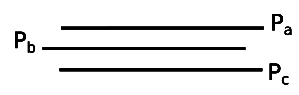
\includegraphics[width=4.5cm]{img/edge-clique.png} & &
    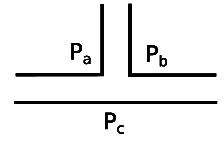
\includegraphics[width=3.5cm]{img/claw-clique.png}%b1EpgTransparenteGrade2
    \\
    \footnotesize %\centering 
    (a)  \footnotesize Representation of a clique as edge-clique. && \footnotesize (b) Representation  of a clique as claw-clique.\\
  \end{tabular}

 \caption{Examples of clique representations.} \label{fig:cliquesRepresentation}
\end{figure}


















% \begin{figure}[h]
%   \centering
%   \begin{tabular}{  p{4cm} p{0.7cm} p{4cm} }
%     %\centering
%     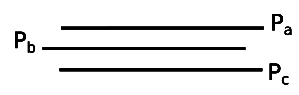
\includegraphics[width=4.5cm]{img/edge-clique.png} & &
%     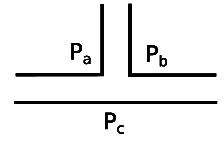
\includegraphics[width=3.5cm]{img/claw-clique.png}%b1EpgTransparenteGrade2
%     \\
%     \footnotesize %\centering 
%     (a)  \footnotesize Representação de uma  clique como clique-aresta. && \footnotesize (b) Representação de uma  clique como clique-garra.\\
%   \end{tabular}

%  \caption{Exemplos de representações de clique.} \label{fig:cliquesRepresentation}
% \end{figure}